\chapter{Data assimilation library based on Kalman filters}


\section{Background}
The Kalman filter is a mathematical method named after Rudolf E. Kalman (\citealt{Kalman1960New}). It uses a system's dynamics model (e.g., physical laws of motion), known control inputs to that system, and measurements (from sensors) to form an estimate of the system's varying quantities (its state) that is better than the estimate obtained by using any one measurement alone. To simultaneously estimate both state variables and parameters, the principle of joint state-parameter estimation is commonly employed, in which the system's state is augmented with its parameters to form a joint state-parameter vector, and this vector is recursively estimated. (\citealt{Chen2008Improved})

\section{Reduced-order unscented Kalman filter (rUKF) and its application to constitutive parameter estimation}
This section is a direct compilation of [\citealt{Xi2010Myocardial}].

\subsection{Estimation of passive material properties via rUKF}
\label{sec-estimator-equation}
In this section, the estimation of the constitutive properties is formulated as the joint state-parameter filtering problem on the mechanical models. We first rewrite the continuum mechanical model in the previous section into its finite dimensional state-space representation, and then formulate rUKF on this system.

\subsubsection{State-space representation of quasi-static nonlinear mechanical model}
\label{sec-state-space-representation-mech-model}

\subsubsection*{Spatial and temporal discretization}
Applying finite element discretization with the cubic-Hermite interpolation for displacement field and trilinear Lagrange interpolation for hydrostatic pressure, the quasi-static nonlinear mechanical model based on the equilibrium equation (\ref{eq-Mechnics-eq4}) is first written as a finite dimensional nonlinear system
\begin{align}
{F^\textnormal{in}}^{(a,j)}(\vect{x}(t),\vect{\theta})= {F^\textnormal{ex}}^{(a,j)}(t), \quad j=1,2,3, \quad a=1,2,\,...\,,N_\textnormal{node},\label{eq-force-quilibrium}
\end{align}
where the terms ${F^\textnormal{in}}^{(a,j)}(\vect{x}(t),\vect{\theta})$  and ${F^\textnormal{ex}}^{(a,j)}(t)$ are given in equations (\ref{eq-equivalent-internal-nodal-force}) and (\ref{eq-equivalent-external-nodal-force}) below. The above equation states that the $j$-th component of the equivalent internal nodal force vector ${F^\textnormal{in}}^{(a,j)}(t)$  at time $t$ and node $a$ of the finite element mesh, as a function of deformed configuration $\vect{x}(t)$ given material parameter $\vect{\theta}$,  is in equilibrium with the equivalent external nodal force vector ${F^\textnormal{ex}}^{(a,j)}(t)$ (\citealt{Bonet1997Nonlinear}). $N_\textnormal{node}$ is the number of total nodes of the geometrical mesh.

The equivalent internal nodal force vector $\vect{F}^\textnormal{in} \in \Real^{3N_\textnormal{node}}$ is given, at node $a$ of the finite element mesh, by
\begin{align}
{F^\textnormal{in}}^{(a,j)}(\vect{x}(t),\vect{\theta})&= \int_{V} T^{MN}(\vect{x}(t),\vect{\theta}) \frac{1}{\det(\tens{F})} \pdpd{x_j}{X_M} \pdpd{\phi_a}{X_N}  dV,  \quad j=1,2,3,\quad a=1,2,\,...\,,N_\textnormal{node}, \label{eq-equivalent-internal-nodal-force}
\end{align}
where the scalar-valued function $\phi_a$, defined over the body volume $V$, is the finite element basis function of node $a$, and $T^{MN}$ is the nine components of the second Piola-Kirchhoff stress tensor, whose dependency on the material parameter vector $\vect{\theta}$ is given by equation (\ref{eq-Mechnics-eq6})--(\ref{eq-Mechnics-eq8}). Similarly the equivalent external nodal force vector $\vect{F}^\textnormal{ex}(t) \in \Real^{3N_\textnormal{node}}$, coming from the external surface force $\vect{s}$, is given by
\begin{align}
{F^{\textnormal{ex}}}^{(a,j)}(t) &= \int_{\partial V} s_j(t) \phi_a  dS, \quad j=1,2,3, \quad a=1,2,\,...\,,N_\textnormal{node}.
\label{eq-equivalent-external-nodal-force}
\end{align}

Given the external forces $\vect{F}^\textnormal{ex}(t)$ at a set of discretized time points \{$t_k, \, k=1,2,\,...\,,K$\}, we solve the nonlinear system (equation \ref{eq-force-quilibrium}) for the deformed configuration $\vect{x}_k $ via applying the Newton-Raphson method, i.e.,
\begin{align}
\vect{x}_k \triangleq \vect{x}(t_k) = G(\vect{F}^\textnormal{ex}(t_k), \vect{\theta}), \label{eq-newtone-solution}
\end{align}
where the operator $G$ denotes the solving process.

\subsubsection*{System equations}
In order to formulate the filtering problem, we will describe the spatially and temporally discretized model (in previous section) with the standard form (equation \ref{quasistatic_system_equation}) of a discrete nonlinear state-space system (\citealt[chapter 6]{Franklin2005Feedback}), in which a system is characterized by the   augmented state vector $\vect{z}$, the system transition operator $f$ (mapping the current state to the future state) and system input vector $\vect{u}$.

We define the external nodal force vector $\vect{F}^\textnormal{ex}(t_k)$ in equation (\ref{eq-newtone-solution}) as the system input vector $\vect{u}_{k-1}$ at time $k-1$, i.e.,
\begin{align}
\vect{u}_{k-1} &\triangleq \vect{F}^\textnormal{ex}_k = \vect{F}^\textnormal{ex}(t_k),
\end{align}
and define the system augmented state vector $\vect{z}_k$ via combining the deformed configuration $\vect{x}$ with the parameter vector $\vect{\theta}$
\begin{align}
\vect{z}_k &= \left( \begin{array}{c}  \vect{x}_k \\  \vect{\theta}_k \\ \end{array} \right) , \label{eq-augmented-state}
\end{align}
where it is assumed that the material parameter is independent of the deformation, i.e.,
\begin{align}
\vect{\theta}_k &= \vect{\theta}_{k-1}. \label{eq-constant-parameter}
\end{align}
Note that although parameter $\vect{\theta}_k$ has no transient itself, it will be recursively changed by the estimator over time.

Combining equation (\ref{eq-newtone-solution}) -- (\ref{eq-constant-parameter}), the nonlinear mechanical system can be described by the following discrete-time, nonlinear system
\begin{align}
\vect{z}_k &= \left( \begin{array}{c} G(\vect{\theta}_{k-1},\vect{u}_{k-1})\\  \vect{\theta}_{k-1} \\ \end{array} \right)  \\
    &= f(\vect{z}_{k-1},\vect{u}_{k-1})  \label{quasistatic_system_equation_no_noise},
\end{align}
where $f$, the system transition operator, is defined by the above equation.

Since the mathematical model is seldom a perfect representation of reality and the parameters for the model are yet to be estimated, the system described by the model (equation \ref{quasistatic_system_equation_no_noise}) has prediction errors. This is represented by the system noise $\vect{w_k}$ as
\begin{align}
\vect{z}_k &= f(\vect{z}_{k-1},\vect{u}_{k-1}) + \vect{w}_{k-1}, \label{quasistatic_system_equation}
\end{align}
where the \emph{white, additive} system noise for $\vect{x}_k$ is assumed to be of Gaussian type with zero mean and constant covariance $\matr{Q}_\textnormal{d}^\textnormal{x}$, and  the system noise for the parameter $\vect{\theta}_k$ has zero mean and constant covariance $\matr{Q}_\textnormal{d}^\theta$, that is,
\begin{align}
\vect{w_k} &\sim \Normal(\vect{0}, \matr{Q}_\textnormal{d}),\\
\matr{Q}_\textnormal{d} &= \left( \begin{array}{cc}  \matr{Q}_\textnormal{d}^\textnormal{x} & \matr{0} \\ \matr{0} & \matr{Q}_\textnormal{d}^\theta \\ \end{array} \right).
\end{align}
Here the subscript d stands for the discrete noise. The magnitude of $\matr{Q}_\textnormal{d}$ (typically a diagonal matrix) reflects our confidence on the model. From the view of efficient implementation of filtering equation in next section, taking into account model noise is not really straightforward in rUKF (nor in any other reduced Kalman) as this introduces the corresponding covariance as an additional term in the covariance matrix $\matr{P}_k^-$ (eq. \ref{eq-analysis-error-covariance}), and the added covariance matrix needs to be reduced (by singular value decomposition) at each filter update. For this issues, we assume the system noise covariance matrix $\matr{Q}_\textnormal{d}$ to be of the same rank as $\matr{P}_k^-$, by introducing a ``fading" parameter in equation \ref{eq-analysis-error-covariance}, and this technique gives satisfactory performance.

\begin{rem}
\label{se-remark-quasitatic}
    We point out that with quasi-static assumption, it is sufficient to write the system equation (\ref{quasistatic_system_equation}) as
    \begin{align}
        \vect{z}_k &= f(\vect{\theta}_{k-1},\vect{u}_{k-1}) + \vect{w}_{k-1},
    \end{align}
    since the augmented state vector $\vect{z}$ at time point $k$ has no dependency on $\vect{x}_{k-1}$ (the deformed configuration at time point $k-1$). This justifies the usage of \emph{reduced-order} filter (described in next section) for estimation of the augmented state vector since the rank of error covariance matrix $\matr{P}_k$ is only of the size of parameter vector $\vect{\theta}$.
    In contrast, for the dynamic systems where the quasi-static assumption does not hold, there is the necessity to apply a first-stage observer (\citealt{Moireau2008Joint}) to essentially reduce the uncertainty of augmented state vector to the parameter space.
\end{rem}

\subsubsection*{Measurement equations}

The measurements $\vect{y}_k \in \Real^{m}$ are given by
\begin{align}
\vect{y}_k &= h(\vect{z}_k)  + \vect{v}_k , \label{eq-measurement}\\
\vect{v}_k &\sim (\vect{0},\matr{R}_\textnormal{d}) , \label{eq-measurement02}
\end{align}
where $h(\vect{z}_k)=h^x(\vect{x}_k)$, and $h^x(\cdot)$ is a operator that maps deformed model configuration $\vect{x}_k$ to its measurements. These measurements are assumed to be corrupted by a noise term $\vect{v}_k$ with zero mean and covariance $\matr{R}_\textnormal{d}$. Assume that we can track the positions of some material points over time, $h^x(\cdot)$ is the linear interpolation matrix that maps all degrees of freedom (coordinates and their spatial derivatives at nodes of the cubic-Hermite mesh) in the model to the coordinates of these material points, that is,
\begin{align}
\vect{y}_k &= \matr{H} \, \vect{z}_k  + \vect{v}_k . \label{eq-measurement03}
\end{align}

\begin{figure}[h!]
\centering
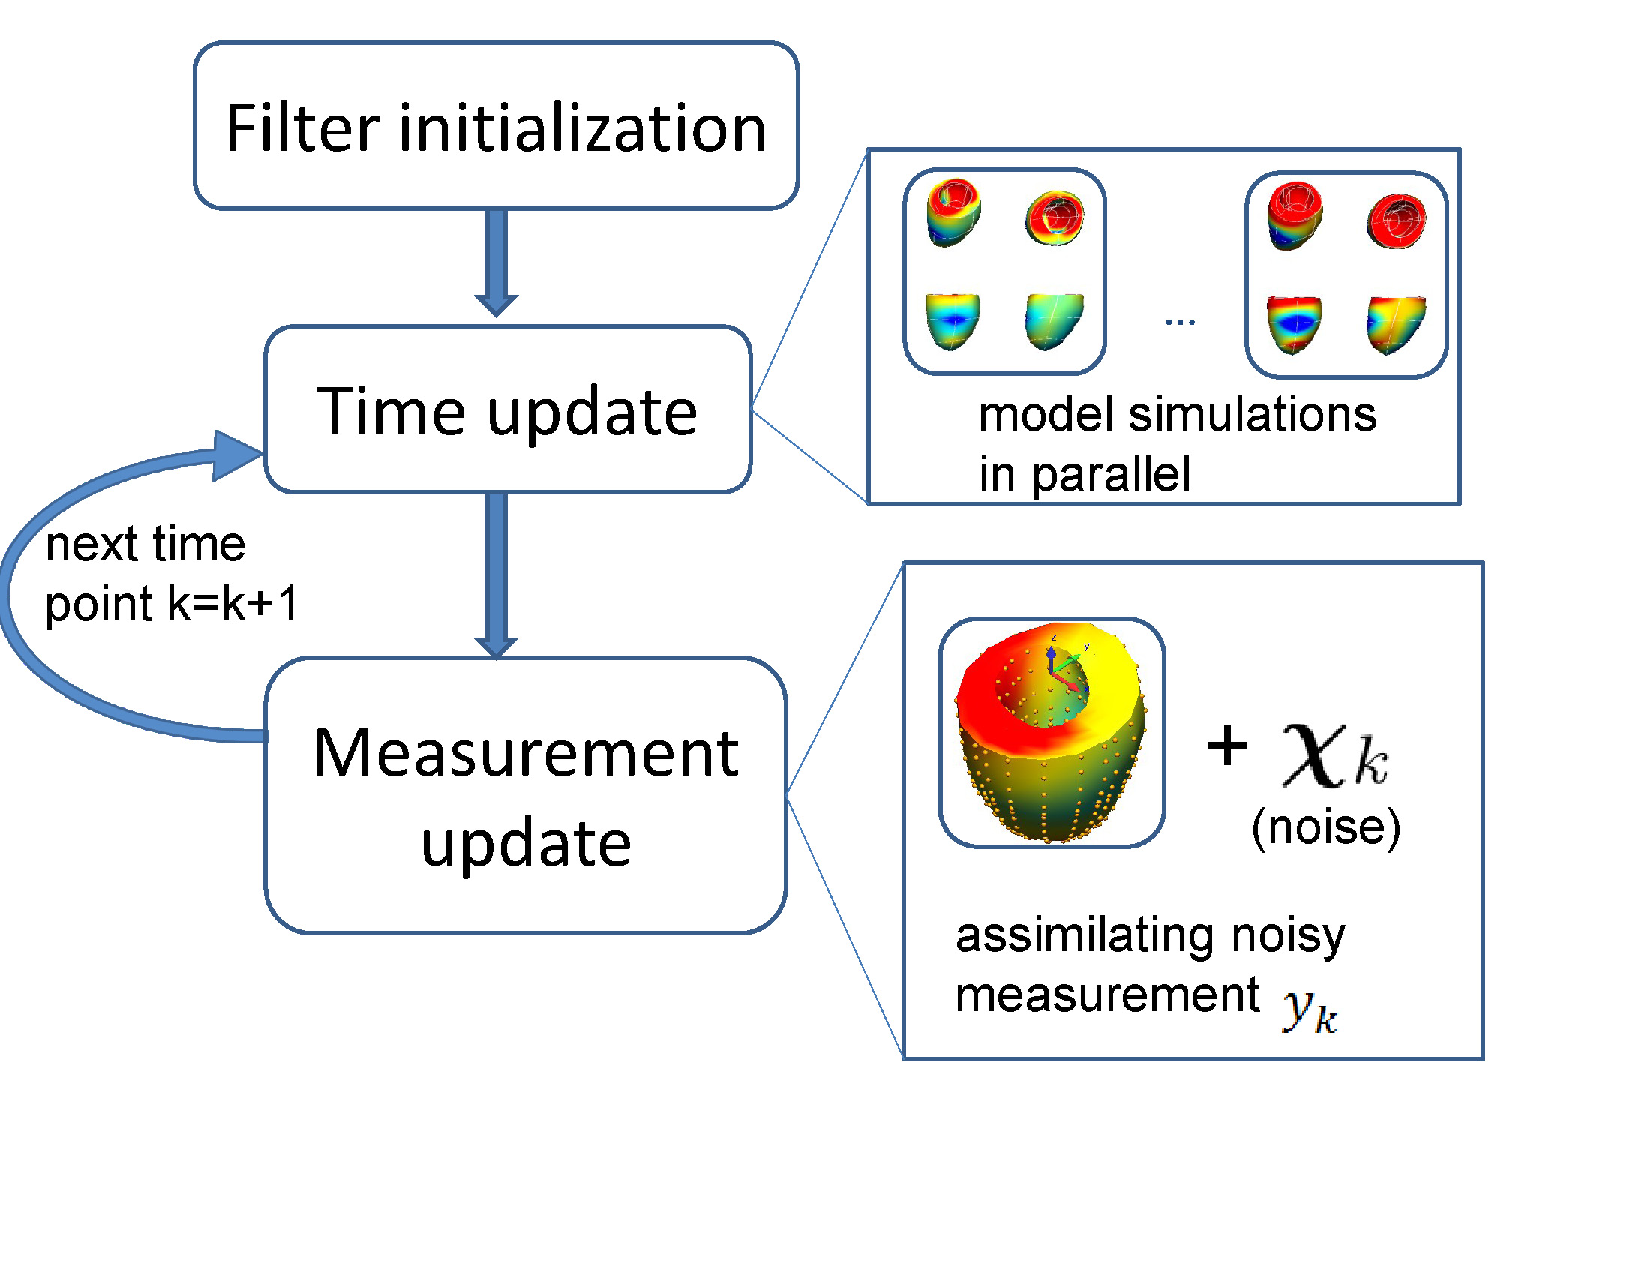
\includegraphics[width=110mm]{ParameterEstimation/2010-08-09-rUKF-estimation-workflow.pdf} %Width: 2001 pixels  Height: 1501 pixels
\caption{Schematic illustration of the estimation procedure via rUKF.}
\label{fig:schmeatic-rUKF}
\end{figure}


\subsubsection{Parameter estimator equations}
\label{sec-parameter-estimation-eq}
Our objective is to estimate constitutive parameters (table \ref{tab-cuccioneLawParameters}) in the mechanical system (eq. \ref{quasistatic_system_equation} and \ref{eq-measurement}) formulated in previous section. This is achieved by applying filtering on estimating the augmented state vector $\vect{z}_k$ (equation \ref{eq-augmented-state}).

%For the filtering on , we adopt rUKF  with canonical unscented transformation to improve estimation accuracy and to avoid possible numerical instability.
%In unscented Kalman filter (UKF), the statistics of a random variable that undergoes a nonlinear transformation is calculated through unscented transformation or sampling at \emph{sigma points}. It is the preferable choice for assimilating measurements into nonlinear systems since it has superior performance than the traditionally used extended Kalman filter (\citealt{Julier1995New}, \citealt[p. 441]{Simon2006Optimal}).

Compared with widely-employed unscented Kalman filter (UKF, \citealt{Julier1995New}), reduced-order UKF (rUKF, \citealt{Moireau2010Reduced}) essentially reduces the rank of the error covariance matrix of the augmented state vector $\vect{z}_k$ from full rank $n_\textnormal{z}$ to $r$, where
\begin{align}
r &\ll n_\textnormal{z}, \quad \vect{z}_k \in \Real^{n_\textnormal{z}}  \textnormal{ (i.e., $n_\textnormal{z}$ is the size of augmented state vector $\vect{z}_k$)}, \label{eq-system-size-01}
\end{align}
and
\begin{align}
r &\ll m, \quad \vect{y}_k \in \Real^{m} \textnormal{ (i.e., $m$ is the size of measurement vector $\vect{y}_k$)}. \label{eq-system-size-02}
\end{align}
With this simplification, the covariance matrix storage is reduced from $n_\textnormal{z} \times n_\textnormal{z}$ to $n_\textnormal{z} \times r$ and the matrix inversion operation can be performed in a subspace $\Matrix^{r \times r}$ instead of $\Matrix^{m \times m}$. Furthermore, the number of model evaluations required by the filter at each time point is also significant decreased, roughly from $O(n_\textnormal{z})$ to $O(r)$. As mentioned in remark (\ref{se-remark-quasitatic}), in the quasi-static systems the uncertainties primarily lie in the parameter space, and thus $r$ can be chosen as the dimension of parameter space, that is
\begin{align}
    r=n_\theta, \quad \vect{\theta}_k \in \Real^{n_\theta} \textnormal{ (i.e., $n_\theta$ is the size of parameter vector $\vect{\theta}_k$)}. \label{eq-system-size-03}
\end{align}


The filtering process consists of three steps (figure \ref{fig:schmeatic-rUKF}) -- initialization of the augmented state vector $\hat{\vect{z}}_{0}^{+}$ and its error matrix $\matr{P}_0^+$, their time updates involving one-step model evaluations, and measurement updates where the noisy data are assimilated based on the relative confidence of the model prediction and measurements accuracy.   In the following notations, we use superscripts $-$ and $+$ to differentiate the prior and posterior estimations (variables before and after assimilating measurements), and $\, \hat{ } \, $  for indicating estimated variables (the mean of the true variable value). Subscript $k$ is the time points with $0$ as the initialization time point.

\subsubsection*{Filter initialization}
For filter initialization, the initial error-covariance $\matr{P}_0^+  \in \Matrix^{n_\textnormal{z} \times n_\textnormal{z}}$, which is typically prescribed as a diagonal matrix with $r$ non-zero elements representing the uncertainties of the system parameters, is decomposed using singular value decomposition (SVD) method
\begin{align}
\matr{P}_0^+ &= \matr{L}_0^+ \matr{\Lambda}_0^+ {\matr{L}_0^+}^T , \label{eq-SEUK-initialization-01}
\end{align}
where $\matr{L}_0^+ \in \Matrix^{n_\textnormal{z} \times n_\textnormal{z}}$ and $\matr{\Lambda}_0^+ \in \Matrix^{n_\textnormal{z} \times n_\textnormal{z}}$ are orthonormal and diagonal matrices respectively.

We keep the first $r$ eigenvectors $\matr{L}_0^+(: \, ,1:r)$ (here this notation denotes the sub-matrix consisting of all the rows and $1$ to $r$ columns of $\matr{L}_0^+$) of $\matr{P}_0^+$, and define its reduced-rank square-root approximation $\matr{S}_0^+ \in \Matrix^{n_\textnormal{z} \times r}$ as
\begin{align}
\matr{S}_0^+ &= \matr{L}_0(: \, ,1:r)\sqrt{\matr{\Lambda}_0^+(1:r,1:r)}. \label{eq-SEUK-initialization-02}
\end{align}
The $r$ column vectors of $\matr{S}$ span the space in which the filter is allowed to make corrections to the augmented state vector $\vect{z}$.

\subsubsection*{Time update}
In time update phase, $2r$ model simulations $f(\hat{\vect{z}}_{k-1}^{+(i)},\vect{u}_{k-1})$ (recall equation \ref{quasistatic_system_equation}) are performed at a set of sampling points $\hat{\vect{z}}_{k-1}^{+(i)}$, in parallel:
\begin{align}
\hat{\vect{z}}_k^{-(i)} &= f(\hat{\vect{z}}_{k-1}^{+(i)},\vect{u}_{k-1}).
\end{align}

These sampling points are referred to as \emph{sigma points} if they are constructed by the so-called \emph{unscented transformation} (\citealt{Julier1997New}). Sigma points are deliberately constructed so that they have the same known statics, e.g., first and second and possibly higher moments, as the given estimate.

While a minimal set of $r+1$ sigma points are adequate to preserve the first and second moments (mean and covariance), we have adopted a \emph{symmetric} set of $2r$-sigma points to improve estimation accuracy, based on the assumption that error processes associated with calibrated measuring devices exhibit the symmetries about a set of principle measurement axes, and such symmetries provide information about the third central moment of the unknown distribution of estimated variables (\citealt{Julier2002Reduced}). We generate the $2r$ sigma points $\hat{\vect{z}}_{k-1}^{+(i)}$ from the reduced-rank square-root approximation matrix $\matr{S}$ by
\begin{align}
\hat{\vect{z}}_{k-1}^{+(i)} &= \hat{\vect{z}}_{k-1}^{+} + \tilde{\vect{z}}_{k-1}^{+(i)},\quad i=1,...,2r, \label{eq-unscented-transformation-01}
\end{align}
where
\begin{align}
\tilde{\vect{z}}_{k-1}^{+(i)}&=\matr{S}^{-}_{k-1}(:,i),\quad i=1,...,r,\label{eq-unscented-transformation-02}
\end{align}
and
\begin{align}
\tilde{\vect{z}}_{k-1}^{+(i)}&=-\matr{S}^{-}_{k-1}(:,i-r),\quad i=r+1,...,2r. \label{eq-unscented-transformation-03}
\end{align}

The statistics (mean $\hat{\vect{z}}_k^{-}$ and error covariance $\matr{P}_k^-$) of the augmented state variable $\vect{z}_k^{-}$ are estimated from the transformed sampling set by
\begin{align}
\hat{\vect{z}}_k^{-} &= \frac{1}{2r} \sum_{i=1}^{2r} \hat{\vect{z}}_k^{-(i)},\\
\matr{P}_k^- &= \frac{1}{\sqrt{2 \rho r}}  \sum_{i=1}^{2r} (\hat{\vect{z}}_k^{-(i)}-\hat{\vect{z}}_k^{-}) (\hat{\vect{z}}_k^{-(i)}-\hat{\vect{z}}_k^{-})^T, \label{eq-analysis-error-covariance}
\end{align}
where $\rho$ (typically $\rho \in [0.9,1]$) is an additional ``fading" parameter to prevent filter divergence through artificially increase the error covariance matrix (\citealt{Brasseur2006SEEK}).

To keep the rank of $\matr{P}_k^-$ to be $r$, we again decompose $\matr{P}_k^-$ as eq. (\ref{eq-SEUK-initialization-01}) and (\ref{eq-SEUK-initialization-02}) to reobtain the  reduced-rank square-root approximation $\matr{S}_{k}^-$ of $\matr{P}_k^-$:
\begin{align}
\opSVD(\matr{P}_k^-) &\to  \matr{S}_{k}^- (\matr{S}_{k}^-)^T.
\end{align}
We point out that the SVD operation in above equation can be computed efficiently without assembling the full $P_k^-$ (\citealt{Moireau2010Reduced}).

\subsubsection*{Measurement update}
Recalling equation (\ref{eq-measurement03}), the observation operator can be adequately written as the observational matrix $\matr{H}$ for our problem. In the measurement update phase, the observation $\vect{y}_k$ is assimilated into the prior estimation $\hat{\vect{z}}_k^-$ to give the posterior estimation based on the \emph{innovation or Kalman gain matrix} $\matr{K}_k$ by
\begin{align}
\hat{\vect{z}}_k^+ &= \hat{\vect{z}}_k^- + \matr{K}_k(\vect{y}_k - \matr{H} \hat{\vect{z}}_k^{-}),
\end{align}
In the above equation, the Kalman gain matrix $\matr{K}_k$ in rUKF can be obtained by applying the matrix inverse lemma (see e.g., \citealt{Simon2006Optimal}) to that for the UKF
\begin{align}
\matr{K}_k &=  \matr{S}_{k}^- (\matr{I} + (\matr{H} \matr{S}_{k}^-)^T \matr{R}_\textnormal{d}^{-1} \matr{H} \matr{S}_{k}^-)^{-1} (\matr{H} \matr{S}_{k}^-)^T \matr{R}_\textnormal{d}^{-1},
\end{align}
where $\matr{R}_\textnormal{d}$ is the measurement error covariance matrix (recall equation \ref{eq-measurement02}). The square-root approximation of error covariance $\matr{S}_{k}$ is updated as
\begin{align}
\matr{S}_{k}^+ &= \matr{S}_{k}^- (\matr{I} + (\matr{H} \matr{S}_{k}^-)^T \matr{R}_\textnormal{d}^{-1} \matr{H} \matr{S}_{k}^-)^{-1/2}.
\end{align}
Note that the matrix inverse and square-root operations in the above equations are performed on $\matr{I} + (\matr{H} \matr{S}_{k}^-)^T \matr{R}_\textnormal{d}^{-1} \matr{H} \matr{S}_{k}^-$ (as mentioned before at the beginning of this section), which reduces the computational cost significantly for large systems.

For further details and formal derivations of the equations in rUKF, please refer to \citet{Moireau2010Reduced}, in particular when the observation operator is nonlinear, which makes the expression of the filter much more intricate. As a summary, rUKF decreases the computational costs dramatically based on the assumption that the rank of error covariance (second order moment) can be reduced. However, filter optimality might be lost because of this simplification, and thus the performance of this filter on our cubic-Hermite interpolation based mechanical model needs to be assessed numerically (see results in the next section), especially with the introduction of measurement noise and exponential-form constitutive law.
